\chapter{Introduction}
\label{chapter:intro}

A computer's processor is an amazing device: it executes millions of instructions each second, at a speed difficult to comprehend. Yet each instruction is very simple and operates on precise data types: read 64 bits from memory address X into register R1, subtract R1 from R2 using unsigned 64-bit integer semantics, etc. For the processor, data is made up of bits and each instruction needs to know the exact size and semantics of its operands, information that allows the processor to decide which logic gates to activate.

On the opposite side of the spectrum, people think in terms of very high-level goals, such as summing up the elements contained in a list. In this high-level goal, there is no mention of what type of elements are contained in the list (integers, floating-point numbers, something else...) or the size and semantics of the result. There are two steps to bridge the gap between a high-level goal and the precise low-level machine instructions necessary to implement it: first, programming languages allow people to express their intent and second, compilers and interpreters translate this intent, written in the source code, into precise low-level machine instructions.

High-level languages such as Python, Scala, Ruby and JavaScript gloss over many implementation details to allow programmers to directly express high-level goals. For example, the following code written in Python sums up a list of numbers:

\begin{lstlisting-nobreak}
 >>> list = [1, 2, 3, 4, 5, `6.0`]
 >>> print `sum(list)`
 21.0
\end{lstlisting-nobreak}

Notice the non-uniform nature of the list: the first five elements are integers while the last is a floating-point number. To allow such code to run, the elements in the list are stored using a uniform representation: each element is a heap-allocated object, with type information attached. Then, to execute the |sum| operation, at each step the next element is inspected and the correct operation is performed based on its type. In this case, the first five additions use integer semantics, followed by a floating-point number addition. % Furthermore, Python automatically adjusts the bit width of integer numbers so operations never overflow. This protects the programmer from the risk of overflows.

Flexibility and abstraction ease programming, but they come at the cost of performance. High-level constructs require long sequences of machine instructions, where data is stored inside heap-allocated objects and operations are executed through indirect calls. These indirections, meant to allow language constructs to handle different use cases are also an important source of slowdowns: values require allocating heap memory while indirect code behaves in unpredictable ways, degrading processor-level optimizations such as caching, prefetching and branch prediction, all of which rely on direct and uniform code patterns. % Compared to their low-level equivalents, which handle precisely one case, high-level constructs can be up to 10$\times$ slower.

Most of the flexibility provided at the language level remains unused in real programs. For example, in practice, it is rather uncommon for a program to store both integers and floating-point numbers in the same list. But, if the language allows it, the low-level code must be prepared to handle it, through indirections.

In statically typed programming languages, generics allow programmers to express the fact that all elements of a list should have the same type. Then, the compiler can check (or infer) the type of elements in the list. In our next example, written in the Scala programming language \cite{scala-odersky}, the compiler decides that the wider 64-bit floating-point type can express all numbers in the list without loss of precision, so it infers the type of |list| to be |List[Double]|:

\begin{lstlisting-nobreak}
 scala> val list = List(1, 2, 3, 4, 5, `6.0`)
 list: `List[Double]` = List(1.0, 2.0, 3.0, 4.0, 5.0, 6.0)
\end{lstlisting-nobreak}

Therefore, the integer values are converted to double-precision (64 bit) floating-point numbers so the list stores only one type of elements\footnote{If the programmer explicitly wants to store the two types of elements, this can be expressed using the |Any| top-level type: |List[Any](1, 2, 3, 4, 5, 6.0)|}. This can be seen in the second line, where the type of the list is inferred to |List[Double]|, signalling the fact that all elements are 64-bit floating-point numbers. This restriction, known at compile-time, has the potential to bring important speed improvements. The same applies to the |sum| operation:

\begin{lstlisting-nobreak}
 scala> println(`list.sum`) // static knowledge: this operation is summing
 21.0                             // up double-precision floating-point numbers
\end{lstlisting-nobreak}

Using the type system to restrict run-time behavior opens the door to using more efficient data representations and faster operations. Yet, the object-oriented model poses unique challenges, which prevent standard compiler optimizations. For example, in the general case, the |sum| operation cannot be inlined and adapted for 64-bit floating-point numbers, as it may be overridden in a subclass of |List|. Therefore, in many cases, object-oriented language compilers forgo the optimization opportunities uncovered by static type systems.

This thesis describes three compile-time approaches that leverage the type system to optimize programs for the data they handle. They were designed from the ground up to support for object-oriented patterns and separate compilation. Together, the three approaches are used in the artifact of the thesis, the miniboxing Scala compiler plugin.

% Employing these transformations allows us to trade flexibility for optimality, by using list objects tailored for 64-bit floating-point numbers and for which the |sum| operation is performed more efficiently. Furthermore, the thesis shows how programmers can manually define more efficient representations for their data, guiding the compiler into using more efficient transformations for the code.

% The problem can be turned around: although |sum| cannot be safely inlined and adapted, nothing prevents its implementation from being already adapted for the type of elements in the list. Since the |sum| implementation is opaque and can be overridden, we can devise a subclass of |List[T]| adapted for double-precision floating-point values. This adapted subclass, also called the specialized variant of |List[T]| for |Double| can only be used when the type of the elements is statically known to be |Double|. But, in exchange, once this is know, the adapted methods and fields can correctly replace the more general versions in |List[T]|.
%
% This approach, called class specialization \cite{iuli-thesis, specialization-iuli}, automates the derivation of variants specialized for primitive types and the program rewriting necessary to introduce them. Based on the static type system guarantees, when the program constructs a list of double-precision floating-point numbers, the compiler can rewrite the class being instantiated by its specialized variant, which offers the exact same methods, with the same signatures. This is what we refer to as ``compatible'' data representation replacement: replacing classes by equivalent, drop-in objects that are adapted for the data they handle.
%
% This is where the thesis begins, by proposing an improved data representation for the specialization transformation.

% Yet, it turns out adapting a |List[Double]| subclass from |List[T]| requires a slightly different transformation: values that were previously stored as |T|, using indirection, are now stored in double-precision floating-point numbers. Yet compatibility with signatures can require that a value, which could be stored as |Double|, is actually passed in as |T|. Therefore, in the process of adapting the class, a different type of data representation transformation occurs: one where the target and its replacement are incompatible, so the compiler needs to introduce coercions.

% \section{Contributions}
%
% In this thesis we study compile-time data representation transformations in object oriented languages, using both compatible and incompatible alternative representations:
%
% % \vspace{-0.5em}
% \begin{itemize}
%   \item[(1)] We devise an efficient data representation for compatible replacements;
%   \item[(2)] We show how compatible replacements ultimately rely on incompatible replacements, and offer an general algorithm for program transformations.
% \end{itemize}
% % \vspace{-0.5em}
%
% We first show that the implementation of the first case relies on the second one and then provide a mechanism that automates the introduction of conversions where necessary.

% Story of development:
%  1. miniboxing
%  2. LDL
%  3. iLDL
\section{Thesis Outline}

The main technical artifact of the thesis is a generics compilation scheme called miniboxing, implemented as a plugin to the Scala compiler, which produces Java Virtual Machine (JVM) bytecode. Miniboxing derives compatible drop-in replacements of generic classes, optimized for primitive types. Then, it automatically introduces these replacements into the code based on type information, improving performance by factors ranging between 1.1 and 20$\times$. In this section we explain how the different chapters of the thesis work together to cover the different aspects of the miniboxing transformation.

\subsection{The Miniboxing Data Representation (Chapter \ref{chapter:miniboxing})}

\begin{wrapfigure}{r}{50mm}
  \centering
  \vspace{-3em}
  \includegraphics[width=50mm]{mbox2-white.pdf}
  \vspace{-3em}
  \caption{Miniboxing Logo}
\end{wrapfigure}

% Generics in the Scala programming language => erasure => boxing
Genericity, also known as parametric polymorphism in functional languages, is a very powerful tool for abstraction: in a statically typed language, it allows defining data structures and algorithms that operate identically for different types of data. For example, the standard linked list class in the Scala library is parameterized on type of its elements: |List[T]| signals that all elements in the list have type |T|. Yet, regardless of the instantiation of |T|, the list preserves the same contract and asymptotic behavior for all its operations. Using generics increases safety, since type-correctness is checked during compilation and promotes code reuse, as the same linked list class can be employed in different contexts, for different types of elements: 32-bit integers, floating-point numbers, strings or any other nested objects or data structures.

However, under the hood, the Java Virtual Machine (JVM) execution platform only supports defining non-generic (monomorphic) classes. Therefore, the generic information in the programming language must somehow be projected onto the less expressive bytecode, producing monomorphic classes. The default solution taken by both the Java and Scala compilers is to use a transformation called erasure \cite{java-erasure}, which compiles a generic class to a single bytecode entity: a monomorphic class where the generic data is stored using references.

Yet, there is a fundamental tension between the different sizes and semantics of the incoming data and the fact that there is a single class which must handle everything. The technical solution taken is to encode primitive types, such as booleans, bytes, integers and floating-point numbers into heap objects, so they can be handled similarly to strings, data structures and other programmer-defined objects. But this operation, known as boxing, is inefficient, introducing indirections and inflating the memory footprint.

% Specialization in Scala => too much bytecode
The first solution to improve generics in Scala, dubbed specialization, was implemented by \textem{Iulian Dragos} \cite{iuli-thesis, specialization-iuli} in 2009: instead of compiling the list into a single bytecode class, specialization creates multiple variants, each adapted for a primitive type. Despite the great speedups brought by this transformation, an important problem soon became apparent: with 10 variants per type parameter, covering the entire Cartesian product of primitives for two or three type parameters produces too many variants. For example, the |Map| class in the Scala library takes two type parameters, so specialization produces as many as $10^2$ variants. Similarly, fully specializing classes such as |Tuple3| and |Function2|, both of which have three type parameters, results in $10^3$ variants. Since all these specialized variants become part of the bytecode, the specialization transformation cannot be used extensively in the Scala standard library, which needs to be keep at a reasonable size.

% Miniboxing => encode everything as a primitive
We begin this thesis where specialization left off: addressing the large number of specialized variants produced when compiling generic classes. Chapter \ref{chapter:miniboxing} presents the miniboxing data encoding, which uses 64-bit long integers to encode primitive values\footnote{We extend the term ``value'' to mean either a final variable (``value'' in the Scala terminology), a variable, an argument or the return of a method. This notation is used consistently throughout the thesis. For immediate constants such as the integer 5 we use the term ``constant'' or ``constant value''.}, regardless of their type. Using this data representation, instead of generating ten variants per type parameter, we only generate two\footnote{In the latest implementation of the miniboxing compiler plugin, version 0.4, the miniboxing transformation generates three variants instead of two, in order to avoid negative interactions with the HotSpot Just-in-time compiler in the Oracle Java Virtual Machine. More information is available on the miniboxing plugin website \cite{miniboxing-www}.}, reducing the amount of bytecode produced. For example, with the miniboxing data encoding, |Map| has just four variants while |Tuple3| and |Function2| each have eight. %Yet, the transformation is more complex than specialization and implementing it required more research breakthroughs.

\begin{figure}[h!]
  \centering
  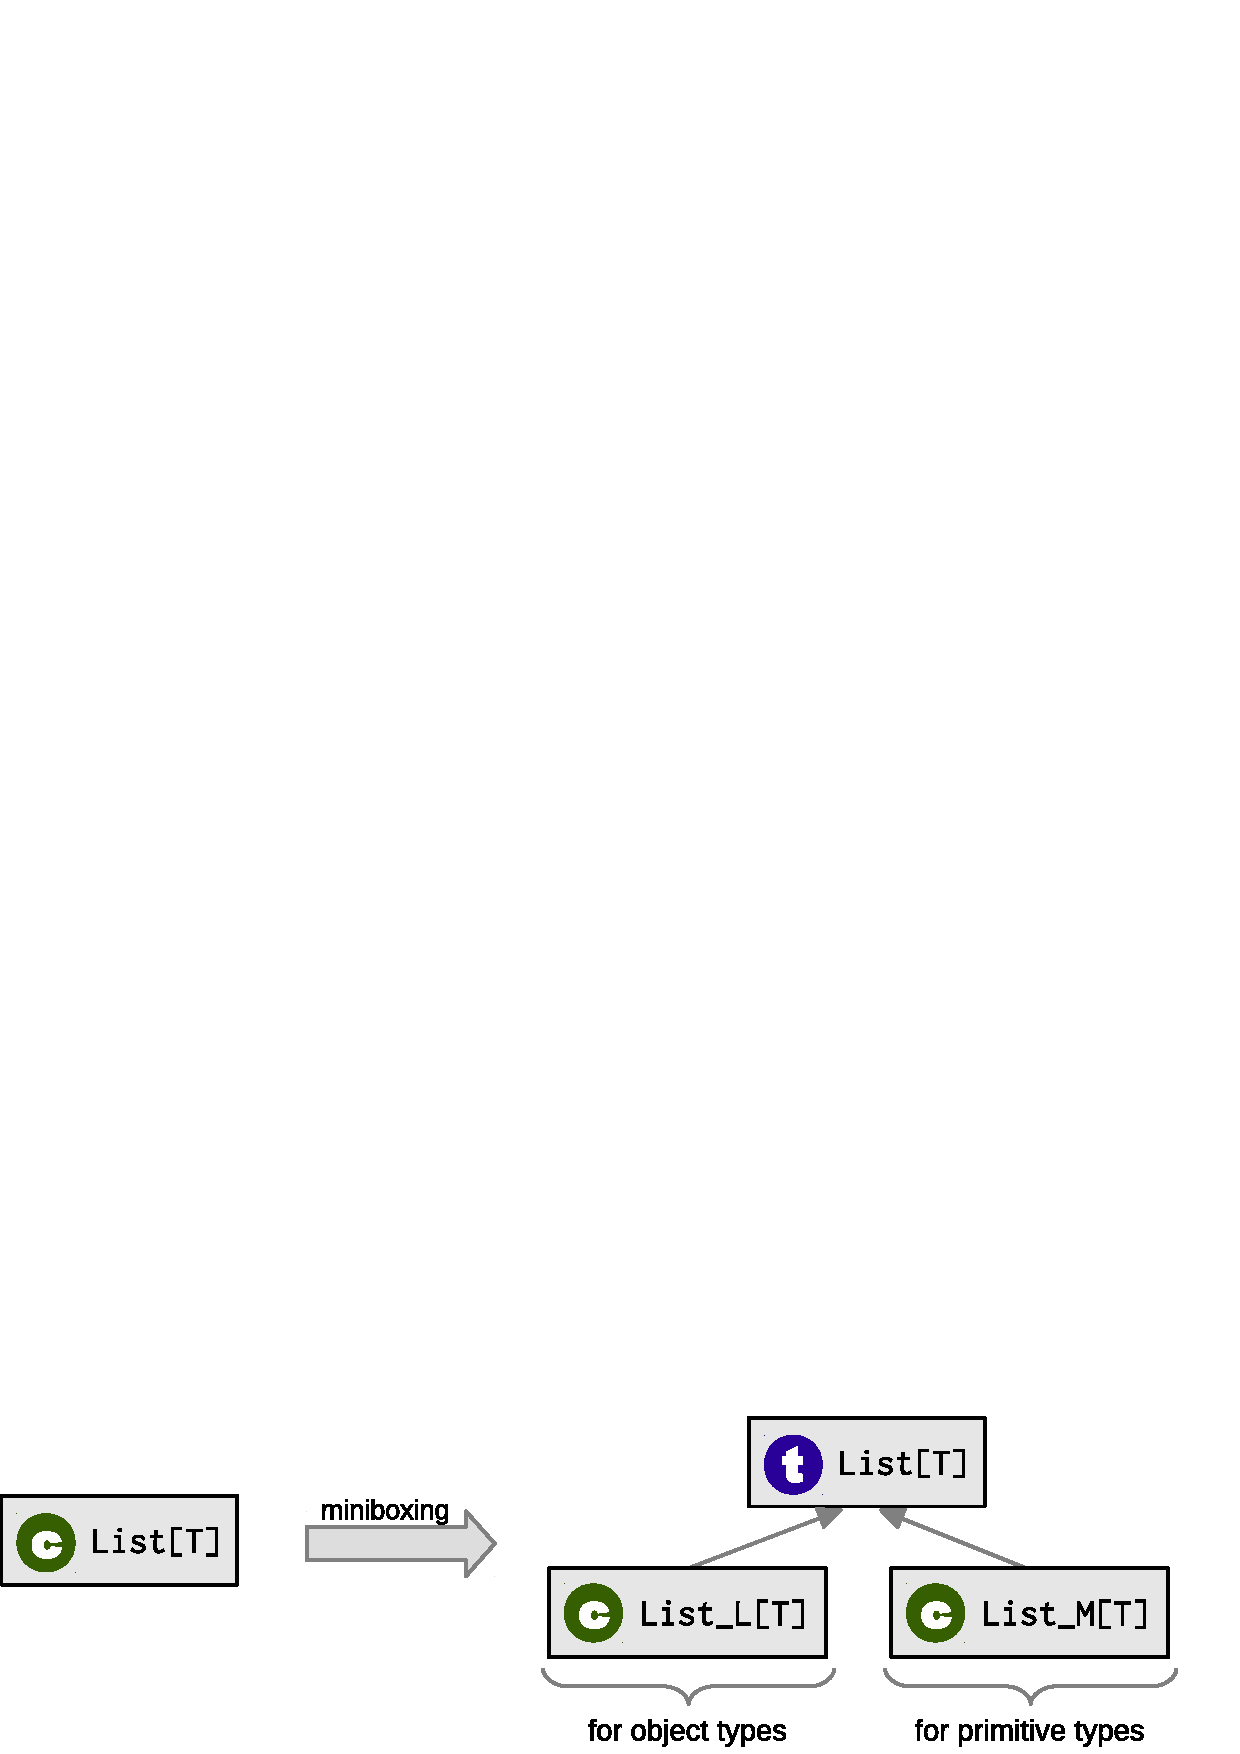
\includegraphics[width=0.8\textwidth]{mbox-diag.pdf}
  \caption{Miniboxing Compatible Transformation}
  \label{fig:mbox-diag}
\end{figure}

% But then T, the type parameter, can be represented as long integers in the ... => LDL
Figure \ref{fig:mbox-diag} shows the two specialized variants of class |List[T]|, automatically generated by the miniboxing transformation. They act as compatible drop-in replacements for the |List[T]| class, and are automatically introduced by rewriting the |new| operator. However, when deriving the code for the |List_M[T]| class there's a different type of data representation transformation taking place: values of type |T|, previously represented as heap objects, are now transformed into 64-bit long integers. These two data representations are not compatible, so, when a value passes from one representation to another the compiler has to introduce conversions.

% In the introduction we mentioned two types of transformations: (1) using compatible drop-in replacements, like specialization and miniboxing and (2) using incompatible replacements, where conversions have to be inserted. In fact, miniboxing, which is a type (1) transformation requires a type (2) transformation behind the scenes: once a class, such as |List[T]|, has been duplicated to create the miniboxed variant, values of type |T| inside it have to be represented as 64-bit long integers. Since the two types, namely |T| and long integer are incompatible, we have to introduce conversions when values pass between representations.

For the initial prototype of miniboxing, the transformation from |T| to long integer was done using the simple and conservative syntax-based transformation described in Section \ref{mbox:sec-mb-traf}. But the problems in scaling this transformation to all the source code patterns expressible in Scala created the need for a better, more principled transformation mechanism. This is how the Late Data Layout mechanism came to be.

% \newpage

% Inspired by the Scala erasure transformation itself, which unboxes scala.Int into the 32-bit ...
\subsection{Late Data Layout (Chapter \ref{chapter:ldl})}

\begin{wrapfigure}{r}{40mm}
  \centering
  \vspace{-2em}
  \includegraphics[width=40mm]{ldl-frog.pdf}
  \vspace{-2em}
  \caption{LDL Logo}
  \vspace{-1em}
\end{wrapfigure}

Late Data Layout (LDL) is a general mechanism for transforming the data representation when the target and its replacement are incompatible. To preserve program consistency, the compiler needs to automatically introduce conversions when values are passed across representations.

The LDL mechanism is inspired by the transformations performed in the Scala compiler backend: The built-in |scala.Int| type corresponds to a 32-bit integer, but it abstracts over the boxed and unboxed representations, exposing fewer decisions to programmers. Then, in the Scala compiler backend, |scala.Int| is transformed to either an unboxed integer (|int| in Java and JVM bytecode) or, as dictated by interactions with other language features, to a boxed one (|java.lang.Integer|). As the transformation progresses conversions between the two representations are introduced in the code as necessary.

Miniboxing and unboxing primitive types in the Scala backend are both instances of LDL transformations. The common pattern handled by LDL is having a high-level type (the type parameter |T| for miniboxing or |scala.Int|) that can be represented in two or more ways. Then, based on the LDL mechanism, the compiler transforms the high-level type into its representations, introducing conversions each time a value is passed across different (and thus incompatible) representations. The LDL mechanism is backed by the type system, which means it is guaranteed to correctly introduce conversions where necessary. Furthermore, LDL allows individually picking the representation of each value in the program, thus allowing fine-grained control over the resulting lower-level code. Finally, special attention was paid to object-oriented code patterns, such as dynamic dispatch, subtyping and interactions with generics, all of which are correctly handled by LDL.

Without going into the implementation details, there are three properties of LDL that stem from its current design:

\begin{itemize}
  \item Selectivity in the choice of data representation, at the level of individual value;
  \item Consistency in terms of passing values between representations; % transformation is provably correct;
  \item Coercion push-down, which reduces the number of coercions executed at runtime
\end{itemize}

Miniboxing makes full use of the three properties, allowing it to offset the code transformation to LDL and focus on the compatible class duplication and replacement problems.

LDL scales beyond miniboxing and unboxing Scala primitive types: it can also drive value class inlining \cite{gosling-value-classes,rose-value-classes-tearing,rose-value-classes-vm} and offer the compiler support for multi-stage programming \cite{tiark-lms, scala-virtualized}. The common trait across these transformations is that the high-level type and its representations are fixed inside the compiler. But this needs not be the case...

%
% Aside from the program transformations shown above, the LDL mechanism can be scaled into a new direction: allowing programers to perform data representation transformations.
%
%
%
% While further developing the miniboxing compiler plugin, we realized there were other transformations necessary to efficiently support the functional aspects of the Scala language, which led to the development of data-centric metaprogramming.

\subsection{Data-Centric Metaprogramming (Chapter \ref{chapter:ildl})}

\begin{wrapfigure}{r}{40mm}
  \centering
  \vspace{-2em}
  \includegraphics[width=40mm]{ildl-frog3.pdf}
  \vspace{-1em}
  \caption{Data-Centric Metaprogramming Logo}
  \vspace{-2em}
\end{wrapfigure}


Data-centric Metaprogramming is an extension of LDL that makes data representation transformations accessible to programmers. Through entities called transformation description objects, programmers can target values of specific (high-level) types and safely replace their data representations by custom, more efficient alternatives. Any type in the language can be targeted, from simple classes all the way to generic nested data structures. The alternative representation is written by the programmer, and it can be based on run-time profiling information or knowledge of how the data is used. Then, once the transformation has been defined, to trigger it,  programmers enclose anything from expressions to entire class definitions inside transformation scopes, where the compiler automatically introduces the custom, improved representation.

% Example:
There are many examples of using data-centric metaprogramming to improve performance:
\begin{itemize}
  \item Improving locality by splitting arrays of records into records of arrays;
  \item Transforming eager collections into lazy collections, achieving deforestation \cite{wadler-deforestation};
  \item Replacing variable-width integers by more efficient fixed-width alternatives;
  \item Specializing a class from a library, which was previously impossible without changing the source code for the class.
\end{itemize}

Of course, programmers still have the possibility to refactor their code by hand instead of using data-centric metaprogramming. Yet, the cost of doing so in large code bases quickly becomes prohibitive and, lacking clear benchmarks, there is no guarantee the refactoring will pay off. Instead, data-centric metaprogramming allows writing idiomatic code which is automatically improved by the compiler, based on the transformation definitions.

% metaprogramming
What makes this extension unique is that it allows programmers to improve the data representation based on their own usage patterns, instead of limiting them to a fixed set of predefined compiler optimizations. This custom nature brings our approach close to metaprogramming. Yet, unlike metaprogramming, where the abstract syntax trees representing the program can be manipulated directly, potentially breaking semantics, data-centric metaprogramming only allows a limited and well-behaved set of transformations that offer correctness guarantees in terms of preserving the object-oriented aspects of the language.

To complete the story, the data-centric metaprogramming approach was actually motivated and used by the miniboxing transformation, in order to efficiently handle the functional aspects of the Scala language. This is explained in the next part.


\subsection{Scaling Miniboxing To Scala (Chapter \ref{chapter:mbox2})}

The last chapter of the thesis presents the technical challenges of scaling the miniboxing transformation to the entire Scala language, with problems such as interoperating with erased and specialized generics and efficient construction and access for core language constructs, such as tuples, functions, arrays and type classes.

\begin{wrapfigure}{r}{40mm}
  \centering
  \vspace{-2.5em}
  \includegraphics[width=40mm]{puzzle.pdf}
  \caption{Miniboxing Component Puzzle}
  \vspace{-2em}
\end{wrapfigure}

In particular, the most interesting part is how a scoped transformation is used to introduce a better function encoding, that allows miniboxed code to efficiently call Scala functions, despite the fact that they use the older  specialization compilation scheme. The function transformation was initially implemented in the miniboxing plugin but we later separated it into the data-centric metaprogramming project. This shows how the three projects have been developed together throughout their existence, with the miniboxing plugin being the technical artifact and Late Data Layout being the underlying transformation.

The next section describes the layers involved in compiling and executing Scala programs and how they are impacted by the miniboxing transformation.

\section{Scala Stack}

\begin{wrapfigure}{r}{60mm}
  \centering
  \vspace{-2.5em}
  \includegraphics[width=58mm]{scala-stack.pdf}
  \caption{Scala Stack}
  \label{fig:scala-stack}
  \vspace{-2em}
\end{wrapfigure}

This thesis has been developed in the context of the Scala programming language with the Java Virtual Machine (JVM) backend, a fact that influences the design decisions in all the techniques presented. Figure \ref{fig:scala-stack} shows the simplified stack, with the additions shown in darker gray. The components are:

The \textbf{Scala source code} is the target of the data representation transformations. At this level, the transformations should have a very limited footprint, ideally consisting only of annotations. As we will see later, the act of marking a class or method as miniboxed or marking a scope as transformed must be persisted at the source level, to allow binary compatibility. Since we expect existing code to be optimized with the techniques presented in the thesis, we avoid any change to the language and the addition of APIs, unless strictly necessary.

The \textbf{compiler} is where most of the changes changes occur, through the plug-in architecture that allows new phases to be injected in the compilation pipeline and existing phases to be skipped. In principle, this allows us to have complete control over the compilation process, from the first to the last phase. This would allow us to emit any output desired, such as the scala.js plugin \cite{scala-js}, which generates its own intermediate representation instead of bytecode. Nevertheless, we limit ourselves to outputting standard JVM bytecode, with the single exception that we persist the high-level Scala signatures in the class file and are able to read them back in the separate compilation scenario. This is a standard feature of the Scala compiler.

The \textbf{runtime/library} layer can include additional runtime support specific to the data representation transformation used. Still, the calls to the runtime support should not be made directly by the programmer but should be introduced automatically by the compiler, based on the source-level annotations.

We assume that both the Scala library and the Java runtime support remain unmodified. Theoretically, the Scala library could be compiled using miniboxing, but for technical and policy reasons, we chose to keep miniboxing as a separate compiler plugin. One of the consequences, seen in Chapter \ref{chapter:mbox2}, is that miniboxing includes optimized implementations of some standard library constructs such as functional interfaces, arrays and type classes.

The \textbf{Java virtual machine} layer receives standard bytecode and is assumed to have a just-in-time (JIT) compiler that performs certain optimizations, such as inlining, loop unswitching and dead code elimination. These are standard optimizations that can be expected of any modern virtual machine. Chapter \ref{chapter:miniboxing} explains exactly how these optimizations impact the performance of miniboxed code.

The layers below, namely the \textbf{operating system} and \textbf{hardware} are automatically abstracted by the virtual machine layer, by offering a uniform API in the runtime/library layer. We are not directly concerned by this layer, although we assume certain common features, such as caching and branch prediction.

Since the most changes occur at the compilation level, the next section describes the language and architecture features that impact the compilation process.

\section{Language Features}

This section describes the language features we support in the modified compilation pipeline. In turn, this motivates the key design decisions in the miniboxing and Data-Centric Metaprogramming projects. The choices in the Late Data Layout mechanism are mostly a consequence of the key decisions in the other projects and the context of the work.

\subsection{Implicit Representation Choice}

The first design goal in both the miniboxing and data-centric metaprogramming projects is to avoid directly exposing representations to the programmer, instead only offering a high-level type. This stems from the desire to reduce the number of decisions a programmer needs to make, assuming this will boost productivity\footnote{Unfortunately we do not currently have rigorous empirical evidence for this assumption.}. However, the opposite choice is equally valid: C++ aims to maintain a one to one relation between the language syntax and the low-level machine code. This means that a computationally expensive operation will require a syntactically more verbose piece of code at the source level. Either approach has its merits: one tries to reduce the decisions while the other improves predictability.

Chapter \ref{chapter:mbox2} shows how performance advisories can be used to counter the unpredictable nature of using high-level types: since the compiler explicitly introduces expensive operations during LDL transformations, it can also warn the programmer, explaining why and where a slowdown is likely to occur. These warnings, coupled with actionable advice on how to avoid the slowdowns can help programmers improve performance even if they do not possess a good understanding of the code base. Section \ref{mbox2:sec:bench} evaluates performance advisories.

In fact, both miniboxing and data-centric metaprogramming could equally be seen as source to source transformations. The miniboxing changes, such as creating class variants and using them where possible could be persisted in the source code. Similarly, the data-centric metaprogramming changes can also be done by programmers. So a natural question is ``Why not allow miniboxing and data-centric metaprogramming do source to source transformations''? Doing so would lower the abstraction level in the code, again forcing the programmer to make more choices (e.g. which variant of the class should I instantiate here?). Therefore we restrict the two transformations to the compiler pipeline.

\subsection{Object Oriented Paradigm}

% Natural paradigm.
% Object-oriented paradigm -- very natural as it follows intensional definitions: genus/differentia definition
%   Example Automobile -- Car, Motorcycle, ..., Tesla (Car with Electric)

% Reuse -
%  -- implementation reuse (List, Vector, Map)
%  -- conceptual reuse (according to Einstein, we know the speed is less than c, which is approximately 1.1*10^9 km/h and above 0), we we use 32-bit integers

Since the work was done in Scala, it takes object orientation as a given. In fact, the object oriented paradigm has the merit of being very close to the natural thought process, specifically to the genus/differentia kind of intensional definitions we usually see in dictionaries: a |Cat| is an |Animal| that meows, the |Dog| is an |Animal| that barks. However, it is exactly this aspect that poses the most challenges: the genus/differentia definitions force the last-moment binding of method implementations, in technical terms dynamic dispatch or virtual calling. Indeed, a big part of the data-centric metaprogramming extension to LDL is dedicated to supporting and emulating dynamic dispatch and to preserving the overriding relationships in the presence of signature changes. These problems would not have occurred in a functional language built on the type classes paradigm.

Another challenge is posed by the imperative aspects in Scala: while the primitive boxing and unboxing operations can be considered side-effect free (considering a managed heap), when allowing the programmer to specify new data representation transformations, we run the risk of affecting semantics. Indeed, this is the subject of Sections \ref{ldl:sec:transform:how} and \ref{ildl:sec:ildl:custom} which explain under which conditions the transformations can be considered semantics-preserving. On the other hand, the evaluation in Section \ref{ildl:sec:benchmarks} clearly shows that slightly bending semantics, in a controlled manner, can actually bring significant performance benefits.

In the transformations we assume a managed heap. Neither miniboxing nor data-centric metaprogramming would work with manual deallocation, since coercions allocate new objects. It may seem like the coercions that ``unbox'' could be used to free the allocated memory, but, in practice, there is no guarantee that the object being unboxed is not aliased somewhere else. We think that the techniques shown in this thesis would work on a region-based \cite{regions} memory management system as well, although we have not tested this.

Depending on the level where reflection is implemented, data representation transformations may or may not affect it. In Scala, there are two levels of reflection: Scala reflection uses types persisted before data representation transformations kick in, and is thus immune to miniboxing and data-centric metaprogramming while the Java reflection, which is implemented at the bytecode level and can observe the transformations that occurred. On the other hand, it is not possible for a program to directly inspect its data representation\footnote{Otherwise we would have a clear case of breaking program semantics.} unless it is using identity-based equality or inspecting the stack.

\subsection{Compile-Time Transformation}

The transformations we are describing take place at compile-time. The implications are that transformations are permanent and that they make their way into the resulting bytecode. Other alternatives include load-time transformations, such as the .NET class specialization \cite{dot-net-generics} and run-time transformations, such as the ones done by Mozilla's \cite{tracemonkey} and Google's virtual machines for JavaScript, the PyPy virtual machine for Python\cite{bolz-pypy-tracing-jit} and the Truffle interpreter framework \cite{truffle}.

Load-time data representation transformations have the merit of avoiding the extra low-level code at the expense of a one-time overhead when a class is loaded. We have experimented with load-time transformations and the conclusion was that, although in theory it is a one-time overhead, keeping the class instantiation overhead-free requires very complex machinery. We present our results in Section \ref{mbox:sec-classloading}.

Run-time data representation transformations have the advantage of being able to speculate on the runtime properties of the data manipulated by the program. This allows them to optimistically optimize the program during just-in-time compilation, while also having the option of undoing an optimization if it proves too optimistic. Run-time data representation transformations are critical for dynamic language virtual machines, where types are not present to limit the possible run-time behaviors and only profiling can uncover optimization opportunities.

\subsection{Open World Assumption and Separate Compilation}

The open world assumption takes a central position in the work presented in this thesis: new classes may be loaded into the system dynamically and all approaches presented support separate compilation, allowing transformations to compose across compilation runs. We explain this topic further in Section \ref{ildl:sec:ildl:separate-compilation}. A closed world approach, despite its drawbacks, would allow much more aggressive optimizations, possibly at the expense of more costly analyses.

\subsection{Binary Compatibility}

Changing the data representation transformation is, by definition, not binary compatible, since it modifies method signatures. This means that updating the data representation in a class or method requires recompiling all its users, so they can also adapt to the transformation. Yet, we do have a weaker binary compatibility guarantee: as long as the data representation transformation is not changed, clients compiled before are binary compatible.

This requires the data representation transformations to be persisted at the source level, through the use of annotations. For example, the miniboxing transformation for a class is triggered by the |@miniboxed| annotation, not by the usage of that class. The reason is that, given different usages of the class that are compiled along with the class, the decision of whether to minibox it may change, rendering previously compiled clients binary incompatible.

Instead, as we show in Chapter \ref{chapter:mbox2}, the miniboxing plugin generates performance advisories when encountering clients that would benefit from miniboxing a class. However, the act of annotating type parameters is done by the programmer and is persisted in the source code.

\section{Contributions}

The thesis makes the following contributions:

\begin{itemize}
  \item It presents the miniboxing generics compilation scheme with (1) its data encoding, (2) its solution to offering compatible drop-in versions of classes and (3) its approaches for interoperating with other generics compilation schemes (Chapters \ref{chapter:miniboxing} and \ref{chapter:mbox2});
  \item It explains Late Data Layout (LDL), a general mechanism for data representation transformations (Chapter \ref{chapter:ldl});
  \item It extends LDL into the data-centric metaprogramming approach, which makes data representation transformations directly accessible to programmers (Chapter \ref{chapter:ildl}).
\end{itemize}

\section{Publications}

The thesis is based on four prior publications:

\begin{itemize}
  \item Chapter \ref{chapter:miniboxing} is based on ``Miniboxing: Improving the Speed to Code Size Tradeoff in Parametric Polymorphism Translations'' (OOPSLA '13) by Vlad Ureche, Cristian Talau and Martin Odersky \cite{miniboxing};
  \item Chapter \ref{chapter:ldl} is based on ``Late Data Layout: Unifying Data Representation Transformations'' (OOPSLA '14) by Vlad Ureche, Eugene Burmako and Martin Odersky \cite{ldl};
  \item Chapter \ref{chapter:ildl} is based on ``Automating Ad hoc Data Representation Transformations'' (OOPSLA '15) by Vlad Ureche, Aggelos Biboudis, Yannis Smaragdakis and Martin Odersky \cite{ildl-tech};
  \item Chapter \ref{chapter:miniboxing} is based on ``Improving the Interoperation between Generics Translations'' (PPPJ '15) by Vlad Ureche, Milos Stojanovic, Romain Beguet, Nicolas Stucki and Martin Odersky \cite{miniboxing-pppj}.
\end{itemize}

\begin{wrapfigure}{r}{20mm}
  \vspace{0.7em}
  \centering
  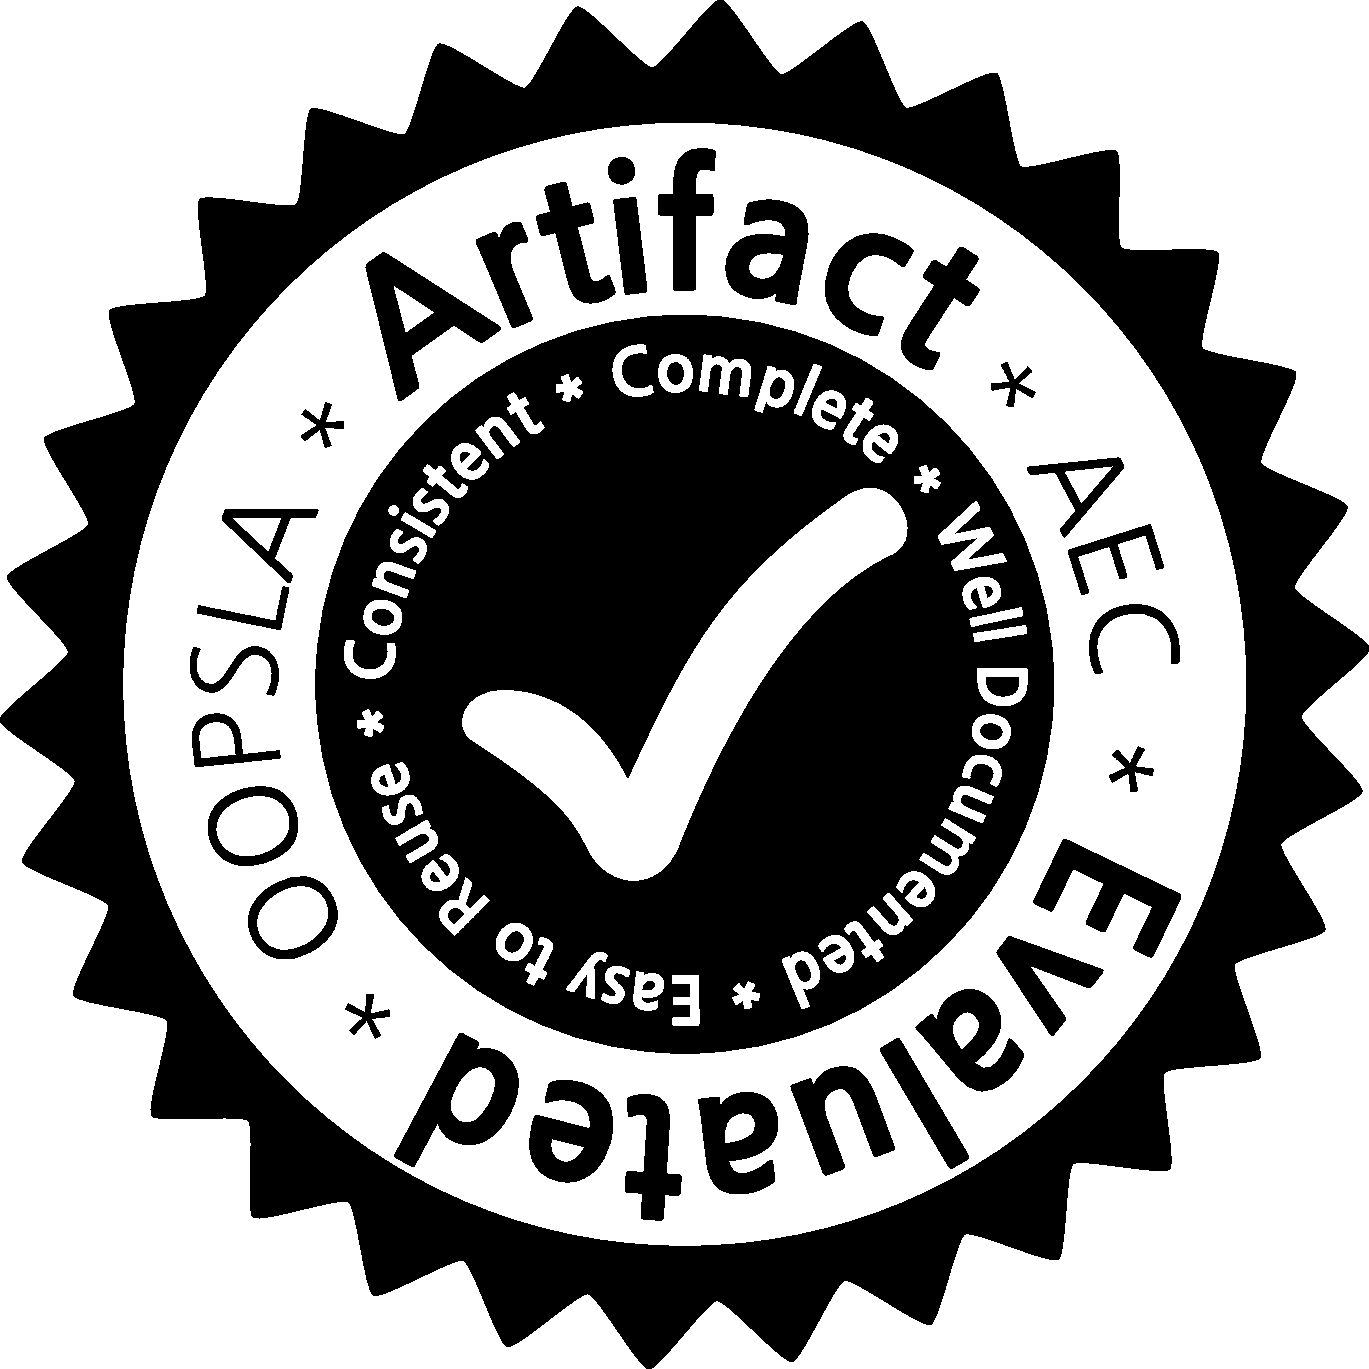
\includegraphics[width=20mm]{aec-badge.eps}
  \vspace{-4em}
\end{wrapfigure}

The papers are used in the thesis with the co-authors' permission.

The implementation artifacts for the first three papers have been checked by the OOPSLA Artifact Evaluation Committee and have received the seal of quality. The PPPJ conference does not offer a similar distinction.
The plugin implementations are openly available: \cite{miniboxing-www,ildl-plugin,ldl-staging-plugin,ldl-value-class-plugin,miniboxing-plugin}.
